% This is the preamble

\documentclass[a4paper]{article}
\usepackage[margin=1in]{geometry}

\usepackage{fancyhdr}
\pagestyle{fancy}
\lhead{Convolution Investigation}
\rhead{\thepage}
\renewcommand{\headrulewidth}{0.4pt}
\renewcommand{\footrulewidth}{0.4pt}

\usepackage{mathtools}
\DeclarePairedDelimiter{\ceil}{\lceil}{\rceil}
\DeclarePairedDelimiter\floor{\lfloor}{\rfloor}

\usepackage[utf8x]{inputenc}
\usepackage{amsmath} % For math formatting
\usepackage{graphicx}
\usepackage{hyperref} 
\usepackage{tcolorbox}
\usepackage{commath}
\usepackage{xcolor}
\hypersetup{
    colorlinks,
    linkcolor={red!50!black},
    citecolor={blue!50!black},
    urlcolor={blue!80!black}
}
\usepackage{multicol}
\usepackage{amssymb}

\newcommand{\op}[2]{#1\{#2\}}

\title{Understanding Convolution}
\author{David Egolf}
\date{September 12, 2016}
% Where the document starts
\begin{document}
\maketitle

\section*{Definition}
The convolution of two sequences $x[n]$ and $h[n]$:
\begin{align*}
(x*h)[n] = \sum_{k=-\infty}^{\infty}x[k]h[n-k]
\end{align*}
Intuitively, we are placing a shifted copy of the sequence $h$ centered at $x = k$, and multiplying this by the $k_{th}$ element in the sequence $x[n]$. We do this for all elements $x[k]$ in the input sequence and add the results.
\\\\
Note that convolution is commutative, distributive, and associative.
\section*{Output of LTI System}
Assume $T$ is a linear time invariant system. Then:
\begin{align*}
\op{T}{\delta[n]} &= h[n] \text{ (impulse response)}\\
\implies \op{T}{x[n]} &= \sum_{k=-\infty}^{k=\infty}x[k]h[n-k]
\end{align*}
\section*{Model Ultrasound System as LTI System}
Consider a single ultrasound transducer, and assume that we use it to transmit a signal, which is then reflected and received by the transducer. Let us define an ultrasound system $U$ that maps from transducer input excitation to the final signal decoded by the transducer:
\begin{align*}
U = T_x \circ M_x \circ R_x
\end{align*}
where $T_x$ is the transmission operator, $M_x$ is the reflection operator (acts like a ``mirror"), and $R_x$  is the receiving operator.
\\\\
If we ignore the transmission delay, and assume that the reflected signal is identical to the transmitted signal up to a change in amplitude, then:
\begin{align*}
\op{M_x}{x[n]} = A \cdot x[n]
\end{align*}
where $A \in \mathbb{R}$.
\\\\
In our simulations we assume that the both $T_x$ and $R_x$ are LTI systems, with the same impulse response. Call this common transducer impulse response $h$. 
\\\\
Using these definitions, we can calculate the output of the ultrasound system:
\begin{align*}
\op{U}{x[n]} &= \op{T_x \circ M_x \circ R_x}{x[n]} \\
&= h[n] *(A \cdot h[n] * x[n]) \\
&= A \cdot \ (h[n] * h[n]) *x[n]
\end{align*}
where we have used the fact that convolution is commutative.
\clearpage
\subsection*{Motivation}
So, in order to understand the action of the ultrasound system, it would be useful to understand the properties of $h[n] * h[n]$, since this is the impulse response of the entire system (up to a scalar multiple).
\section*{Problem Statement}
Investigate the properties of  the self convolution $(h*h)[n]$ of a sequence $h: \mathbb{Z} \rightarrow \mathbb{R}$, in the context of an ultrasound system.
\section*{Solution}
\subsection*{Causal}
I assume there is no noise in the ultrasound system to be modeled. I assume that in a noise free ultrasound system, the system will not begin to transmit data prior to excitation, and the system will not begin to receive data prior to a transmitted signal hitting the receiver. Therefore:
\begin{align*}
h[n] = 0 \text{ for } n < 0 \implies (h*h)[n] = 0 \text{ for } n < 0 
\end{align*}
This implies that the LTI system  $h*h$ is causal. 
\subsection*{Stable}
I assume that if we stop exciting the transducer, then after a finite amount of time the ultrasound receiver will stop receiving anything. That is:
\begin{align*}
(h*h)[n] = 0 \text{ for } n \geq N
\end{align*}
This implies that we are working with a finite impulse response system, and therefore the system is stable.
\subsection*{Not Memory-less}
The output $y[n]$ depends on all values of the input $h[n]$, not just the current value of $n$. Therefore, the system is not memory-less.
\subsection*{Equation for Output}
The output of the system $(h*h)[n]$ is explicitly:
\begin{align*}
(h*h)[n] &= \sum_{k=-\infty}^{\infty}h[k]h[n-k]
\end{align*}
Since the system is causal, we only need to sum over the terms where $k \geq 0$ and $n - k \geq 0 \implies k \leq n$:
\begin{align*}
(h*h)[n] &= \sum_{k=0}^{n}h[k]h[n-k]
\end{align*}
To get some intuition, we write out this sum explicitly in the case when $h[0] = 1, h[1] = 2, h[2] = 3, h[3] = 4, h[4] = 5$ and $h[j] = 0$ for all other $j \in \mathbb{Z}$:
\begin{align*}
(h*h)[n] &= h[0]h[n] + h[1]h[n-1] + h[2]h[n-2] + h[3]h[n-3] + h[4]h[n-4]
\end{align*}
\clearpage
\subsection*{Nonzero Output Region As Function of Length}
Let $L$ be an integer called the ``length" of the impulse response. We provide elements $h[0], h[1], ..., h[L-1]$ to MATLAB when specifying the impulse response. We require $L \geq 1$ and $h[n] = 0$ for all $n \geq L$.
\\\\
We assume that our impulse response starts at zero and ends at zero, so set $h[0] = h[L-1] = 0$.
\\\\
Using this information, we can rewrite the form of the output $(h*h)[n]$. We are interesting in determining exactly at which times the output can be nonzero. The output $(h*h)[n]$ will be zero at $n$ if:
\begin{align*}
h[k]h[n-k] = 0 \text{ for } k = 0,1,..,n
\end{align*}
Since we assume $h[0] = 0$ and $(h*h)[n] = 0$ for all $n \geq L -1$, we can reduce the number of terms under consideration. Specifically, if $n \geq L-1$, then the output is zero, and if $n \leq 0$ then the output is zero. So, it remains to consider the cases in which $1 \leq n \leq L -2$. These are the only cases in which would possibly get nonzero output.
\\\\ 
We can further restrict these cases by realizing that if $L \leq 2$, then the entire sequence is zero and so the output will be zero. So, we only need to consider the cases $1 \leq n \leq L -2$ where $L \geq 3$. We want to know for which of these $n$ values we have a chance for nonzero output, as a function of $L$ (clearly the maximum $n$ for nonzero output will increase with $L$).
\\\\
Our strategy is to start small and search for a pattern:
\\\\
If $n = 1$:
\begin{align*}
h[k]h[n-k] = h[k]h[1-k]
\end{align*}
Since $1 - k \leq 0$ for $k = 1,..,L-2$, the output is always zero in this case. As a result, we only need to consider the possible nonzero cases as consisting of $2 \leq n \leq L -2$.
\\\\
If $n = 2$:
\begin{align*}
h[k]h[n-k] = h[k]h[2-k] \\
\end{align*}
The possible nonzero $h[i]$ range is $i = 1,2..,L-2$. Checking when we are in this range:
\begin{align*}
1 \leq 2-k \leq L -2 \\
\implies k &\leq 1 \text{ and}\\
\implies 4 &\leq L + k \implies k \geq 4 - L \\
\text{Together: } \\
4 - L \leq k \leq 1
\end{align*}
In order to satisfy this inequality, we need:
\begin{align*}
4 - L \leq 1 \implies L \geq 3
\end{align*}
We also need:
\begin{align*}
4 - L  \leq k_{max}, 1  \geq k_{min}
\end{align*}
Where $k_{max}$ is the largest value $k$ can take on, and $k_{min}$ is the smallest value $k$ can take on, while preserving the fact that $h[k]$ might be nonzero. From our work before, $k_{max} = L - 2$ and $k_{min} = 1$.
\\\\
So, we need:
\begin{align*}
4 - L \leq L -2, 1 \geq 1 \\
\implies 2L \geq 6 \implies L \geq 3
\end{align*}
\\\\
So, $(h*h)[2]$ has a chance to be nonzero when $L \geq 3$.
\clearpage
Let's generalize this argument, setting $n = a$:
\begin{align*}
h[k]h[n-k] = h[k]h[a-k] \\
\end{align*}
The possible nonzero $h[i]$ range is $i = 1,2..,L-2$. Checking when we are in this range:
\begin{align*}
1 \leq a-k \leq L -2 \\
&\implies k \leq a - 1 \text{ and}\\
&\implies a + 2 \leq L + k \implies k \geq a + 2 - L \\
\text{Together: } \\
a + 2 - L \leq k \leq a - 1
&\implies L \geq 3
\end{align*}
We also need:
\begin{align*}
a + 2 - L  \leq k_{max}, a - 1  \geq k_{min}
\end{align*}
Where $k_{max}$ is the largest value $k$ can take on, and $k_{min}$ is the smallest value $k$ can take on, while preserving the chance that $h[k]$ might be nonzero. From our work before, $k_{max} = L - 2$ and $k_{min} = 1$.
\\\\
So, we need:
\begin{align*}
a +2 - L \leq L -2,~a-1 \geq 1 \implies a \geq 2 \\
\implies 2L \geq a + 4 \implies L \geq \frac{a+4}{2}
\end{align*}
\\\\
Substituting $n = a$, we find $(h*h)[n]$ has a chance to be nonzero when $L \geq \frac{n+4}{2}$ and when $n \geq 2$.
\\\\
\subsection*{Largest and Smallest Nonzero $(h*h)[n]$}
Using this information, we can find the first possibly nonzero term. Trying $n = 2$, the condition for the output to be nonzero is:
\begin{align*}
L \geq \frac{2+4}{2} = 3 \implies L \geq 3
\end{align*}
So, $n = 2$ is the smallest value of $n$ for which $(h*h)[n]$ is possibly not zero. 
\\\\
Next, let's find the largest $n = n_{max}$ for which $(h*h)[n]$ is possibly nonzero. We know that this $n \geq 2$. Also, for $(h*h)[n_{max}]$ to be possibly nonzero, we need:
\begin{align*}
2L \geq n_{max} + 4 \\ 
\implies n_{max} \leq 2L - 4
\end{align*}
Choosing the largest element in this set, we get $n_{max} = 2L -4$.
\\\\
So, $(h*h)[n]$ is possibly nonzero for $2 \leq n \leq 2L-4$.
\subsection*{Properties of $h*h$ So Far}
Adding this new information about the nonzero range for $n$:
\begin{align*}
(h*h)[n] = \sum_{k=0}^{n}h[k]h[n-k] \text{ (possibly nonzero for } 2 \leq n \leq 2L-4) 
\end{align*}
This system is LTI, causal, stable, and not memory-less.
\clearpage
\subsection*{Lack of Symmetry in Self Convolution}
It turns out that the convolution of a sequence with itself is NOT symmetric (doesn't form a palindrome when written out), even though the autocorrelation of a sequence with itself is! For example, if $h = [0,1,2,0]$ (starting at $n = 0$), then:
\begin{align*}
(h*h)[0]& = \sum_{k=0}^{0}h[k]h[0-k] = h[0]h[0] = 0 \\
(h*h)[1] &= \sum_{k=0}^{1}h[k]h[1-k] = h[0]h[1] + h[1]h[0] = 0 \\
(h*h)[2] &= \sum_{k=0}^{2}h[k]h[2-k] = h[0]h[2] + h[1]h[1]+h[2]h[0]= 0 + 1 + 0 = 1 \\
(h*h)[3] &= \sum_{k=0}^{3}h[k]h[3-k] = h[0]h[3] + h[1]h[2]+h[2]h[1]+h[3]h[0]= 0 + 2 + 2 + 0 = 4 \\
(h*h)[4] &= \sum_{k=0}^{4}h[k]h[4-k] = h[0]h[4] + h[1]h[3]+h[2]h[2]+h[3]h[1] + h[4]h[0]= 0 + 0 + 4 + 0 = 4 \\
\end{align*}
And since $n_{max} = 2L-4 = 4$, $(h*h)[n] = 0$ for all larger $n$.
\subsection*{Sufficient Condition for Symmetry in Self Convolution}
The autocorrelation of a sequence is known to be symmetric. The autocorrelation for a real sequence is:
\begin{align*}
ACF(h[n]) = \sum_{k=-\infty}^{\infty}h[k]h[k-n]
\end{align*}
For comparison, here is the the definition of a sequence convolved with itself:
\begin{align*}
(h*h)[n] &= \sum_{k=-\infty}^{\infty}h[k]h[n-k] \\
&= \sum_{k=-\infty}^{\infty}h[k]h[-(k-n)]
\end{align*}
If we assume that $h[n]$ satisfies $h[n] = h[-n]$ (it is symmetric in time), then $h[-(k-n)] = h[n-k]$ and we find $ACF(h[n]) = (h*h[n])$ in this case. So, a time symmetric sequence $h[n] = h[-n]$ has a symmetric self convolution.
\subsection*{Incorporating Sinusoidal Shape}
The impulse function $h[n]$ we use in simulation is of the form:
\begin{align*}
h[n] = a[n]\sin(w \cdot n)
\end{align*}
where $a[n]$ is a sequence of real numbers and $w \in \mathbb{R}$. I assume that we use  a natural number $m$ of cycles (in order to ensures that $h[0] = h[L-1] = 0$ and also to produce an output that integrates to zero - which helps reduce side lobe energy). This tells us the value of $w$:
\begin{align*}
w \cdot (L-1) = 2 \pi m \\
\implies w = \frac{2 \pi m}{L-1}
\end{align*}
So, the impulse $h[n]$ is of the form, where $m \in \mathbb{N}$ is the number of cycles used:
\[
 h[n] =
  \begin{cases} 
      \hfill a[n]\sin(\frac{2 \pi m}{L-1} \cdot n)   \hfill & 0 \leq n \leq L -1 \\
      \hfill 0 \hfill & \text{ for all other $n$} \\
  \end{cases}
\]
\clearpage
\subsection*{Consequences of Sinusoidal Shape}
For simplicity, we begin by assuming $a[n] = 1$ for all $n$. MATLAB evidencce seems to suggest that with the additional assumption of sinusoidal shape, the impulse response of the ultrasound system $h*h$ is now symmetric:
\begin{center}
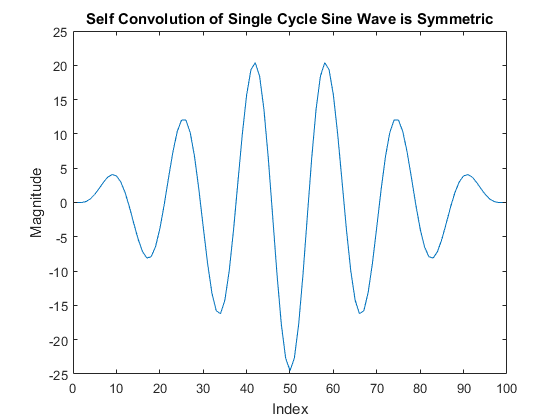
\includegraphics[scale=1]{symmConvSin.png}
\end{center}
The most immediate symmetry present in an impulse response of this form is as follows:
\begin{align*}
h[a] = -h[L-1 - a]~\forall a \in \mathbb{Z} \\
\implies 
h[a-u] = -h[L-1 - (a-u)] = -h[L-1 - a + u)]
\end{align*}
(ASSUMED FOR NOW)
\\\\
If a sequence has this symmetry, it its self convolution symmetric? That is, we want to show:
\begin{align*}
(h*h)[2 + a] &= \sum_{k=0}^{2+a}h[k]h[2+a-k] = (h*h)[2L-4- a] = \sum_{k=0}^{2L-4-a}h[k]h[2L-4-a-k] \\
\iff
\sum_{k=0}^{2+a}h[k]h[2+a-k] &= \sum_{k=0}^{2L-4-a}h[k]h[2L-4-a-k]
\end{align*}
Define $u$ so that $k = L -1-u$. Then $h[k] = h[L -1-u] = -h[u]$, and $2L -4 -a -k = -a+L+u-3$. Since $u = L-k-1$, if $k = 0$ then $u = L - 1$. If $k = 2L-4-a$ then $u = a-L+3$:
\begin{align*}
\iff \sum_{k=0}^{2+a}h[k]h[2+a-k] &= \sum_{u=L-1}^{a-L+3}h[L-1-u]h[L-3-a+u] &= \sum_{u=L-1}^{a-L+3}-h[u]h[L-3-a+u]
\end{align*}
Rewriting the second part of the second sum:
\begin{align*}
h[L-3-a+u] = h[L-1-a+(u-2)] = -h[a-(u-2)] = -h[2+a-u]
\end{align*}
Plugging this back in, renaming $u$ to $k$, and continuing the same chain of implications:
\begin{align*}
\iff \sum_{k=0}^{2+a}h[k]h[2+a-k] &= \sum_{k=L-1}^{a-L+3}h[k]h[2+a-k]
\end{align*}
Call $A = 2+a$:
\begin{align*}
\iff \sum_{k=0}^{A}h[k]h[A-k] &= \sum_{k=L-1}^{A-(L-1)}h[k]h[A-k]
\end{align*}\
We want to show that this relationship holds for all integers $A$.
\\\\
Based on experiments in MATLAB, it appears that the right side contains all the same nonzero terms in the sum as does the left side (and it may have more or less zero terms). We try to show that the right and left side have the same nonzero terms.
\\\\
We need to deal with the case where $2 \leq A \leq 2L -4$, since the two sides are both zero for other values of $A$. To show this, consider the case in which $A$ is outside of this range. In this case, then clearly the left handside $(h*h)[A] = 0$. The righthand side is $(h*h)[2L-4-a]$, and so if $-a > 1$, the righthand side is zero. Now $-a>1 \implies a > -1 \implies A -2 > -1 \implies A > 1$. So we need $A  \geq 2$ for the righthand side to be possibly nonzero. Also, since the righthand side is $(h*h)[2L-4-a]$, if $2L-4-a \leq 1$ then the righthand side is zero. To make the righthand side nonzero we therefore need $2L-4-a \geq 2 \implies 2L-4-(A-2) \geq 2 \implies 2L -4 \geq A$. So, for the righthand side to be possibly nonzero we need $2 \leq A \leq 2L-4$. If $A$ is not in this range, the two sides are equal. Also note that we only need to check for $L \geq 3$, since the output is otherwise always zero.
\subsubsection*{Simple Case Investigation}
Our strategy is to look at a simple case, and then generalize. \\
If $A = 2$, we get (LHS):
\begin{align*}
\sum_{k=0}^{2}h[k]h[2-k] = h[0]h[2] + h[1]h[1] + h[2]h[0] = h[1]h[1]
\end{align*}
For the RHS, we get:
\begin{align*}
\sum_{k=L-1}^{2-(L-1)}h[k]h[2-k] = \sum_{k=2-(L-1)}^{L-1}h[k]h[2-k]
\end{align*}
We only need to sum over $k \geq 1$. Since $2-(L-1) < 1$ (for $L \geq 3$ - the output is always zero otherwise), we can start summing at $k = 1$:
\begin{align*}
\sum_{k=2-(L-1)}^{L-1}h[k]h[2-k] = \sum_{k=1}^{L-1}h[k]h[2-k]
\end{align*}
We also require $2-k \geq 1$ to get a possibly nonzero output. This implies we only need to sum up to when $k = 1$:
\begin{align*}
\sum_{k=2-(L-1)}^{L-1}h[k]h[2-k] = \sum_{k=1}^{1}h[k]h[2-k] = h[1]h[1]
\end{align*}
And so the left and right side match in this case.
\clearpage
\subsubsection*{Generalizing}
We now try and show this result holds for all integers $A$:
\begin{align*}
\sum_{k=0}^{A}h[k]h[A-k] &= \sum_{k=L-1}^{A-(L-1)}h[k]h[A-k]
\end{align*}
Our idea is to remove any terms that will always be zero from each side. Keep in mind that there is only a possibility of nonzero terms when $2 \leq A \leq 2L -4$.
\\\\
On both sides, we want to include all nonzero terms when summing $\sum_{-\infty}^{\infty}h[h]h[A-k]$. A term is possibly nonzero if $1 \leq k \leq L - 2$ and $1 \leq A - k \leq L -2$. This means we need to sum exactly the terms that satisfy the following conditions:
\begin{align*}
k &\geq 1 \\
k &\leq L-2 \\
k &\leq A \\
k &\geq A - L + 2
\end{align*}
The sum on both sides should be:
\begin{align*}
\sum_{k=\max(1,A-L+2)}^{\min(A,L-2)}h[k]h[A-k] 
\end{align*}
However, including extra terms doesn't hurt. The left side is clearly equal to this sum. It sums starting a $k = 0$, while the first needed index is at least 1. It stops summing at $A$, and $A \geq \min(A,L-2)$.
\\\\
It remains to show that the sum on the right side also has the same value as the general form. There are two major cases to consider: when $L-1 < A-(L-1)$ and when $L - 1 \geq  A-(L-1)$.  We also have to consider when $L -1 = A-(L-1)$.
\\\\
Let us begin by considering the case $L-1 < A -(L-1) \implies A > 2L - 2 \implies A - L +2 > L$. Since $L \geq 3$, then $A - L + 2 > 3$. So, $\max(1,A-L+2)$ in this case is $A-L+2$. Also, since $A-L+2 > L$, then $A-L+2 > L -1$ and so $\max(1,A-L+2) > L - 1$ in this case. That means the right side starts at a small enough summation index. Considering the upper index in this case, we need to know the minimum of $A$ and $L-2$. Now, $L-1 < A -(L-1) \implies L+(L-2) < A \implies \min{(A,L-2)} = L-2$. Also, since we just saw $A-(L-1) > L - 1 > L - 2 = \min{(A,L-2)}$, the right side ends at a large enough summation index.
\\\\
Now we consider the case $A-(L-1) < L - 1$. We start summing at $k = A -(L-1)$ and stop summing at $k = L -1$. We need to make sure $A-(L-1) \leq \max(1,A-L+2)$. Clearly $A-L+1 < A-L+2 \implies A-(L-1) \leq \max(1,A-L+2)$. We also need to make sure that $L-1 \geq \min(A,L-2)$ in this case. Since $L -1 > L - 2$, $L-1 \geq \min(A,L-2)$.
\\\\
Finally, we consider the case in which $L-1 = A-(L-1) \ A = 2L-2$. However, we already proved the two sides were equal for $A \geq 2L-4$.
\clearpage
\section*{Alternate Proof: \\ Symmetric Self Convolution for Symmetric Enough Sequences}
\subsection*{Self Convolution Operator Shape Invariance Under Time Shift}
Consider an arbitrary sequence $h: \mathbb{Z} \rightarrow \mathbb{R}$. Define an operator $T$, ``the self convolution operator", so that:
\begin{align*}
\op{T}{h}[n] = (h*h)[n]
\end{align*}
We want to show that as the input is shifted, the output is shifted but preserves its shape. Define a shifted input as $h_1[n] = h[n-n_0]$.
\\\\
Seeing if this definition is met:
\begin{align*}
\op{T}{h_1}[n] = (h_1*h_1)[n] =  \sum_{k=-\infty}^{\infty}h_1[k]h_1[n-k] = \sum_{k=-\infty}^{\infty}h[k - n_0]h[n-k-n_0]
\end{align*}
Setting $u = k - n_0 \implies k = u + n_0$:
\begin{align*}
\op{T}{h_1}[n] =  \sum_{u=-\infty}^{\infty}h[u]h[n-(u+n_0)-n_0] =\sum_{u=-\infty}^{\infty}h[u]h[n-2n_0 -u] = \op{T}{h}[n-2n_0]
\end{align*}
And so the shape stays the same as the input changes. Therefore, if $h[n]*h[n]$ has a symmetric shape about some point if and only $h[n-n_0]*h[n-n_0]$ has a symmetric shape about some point.
\subsection*{Time Shifting the Signal to be Odd About Origin}
We are interested in the self convolution of the signal $h[n]$, which is possibly nonzero for $1 \leq n \leq L -1$, but is otherwise zero. In addition, $h[n] = -h[L-1-n]$ for all integers $n$. Assume that $h$ has an odd number of possibly nonzero values: $L$ is odd. Then we can shift $h$ so that it has odd symmetry. Calling this shifted version $g$, we have $g[-n] = -g[n]$ for all integers $n$.
\\\\
Specifically, if $L$ is odd, then we want to shift the center of the new sequence to be at $(L-1)/2$. So, $g[n] = h[n+(L-1)/2]$. This new sequence $g[n]$ is odd about $n = 0$. Since it is  a shifted version of $h[n]$, its self convolution will be a shifted copy of the self convolution of $h[n]$. We now compare the self convolution of $g[n]$ to its autocorrelation:
\begin{align*}
(g*g)[n] = \sum_{k = -\infty}^{\infty} g[k]g[n-k] \\
ACF(g)[n] = \sum_{k = -\infty}^{\infty} g[k]g[k-n] 
\end{align*}
However, $g[n-k] = -g[k-n]$ by the nature of our construction. Therefore, in this case we can relate self convolution and autocorrelation:
\begin{align*}
-(g*g)[n] = ACF(g[n])
\end{align*}
Since the autocorrelation of a sequence is symmetric about a point, so must the self-convolution in this case.  This shows that sequences $h[n]$ of the form used as the impulse response for our ultrasound system have a self convolution symmetric about a point. In addition, it shows that the peak of the self convolution must be negative. Indeed, the earlier plot of self convolution has a negative peak.
\\\\
In general, for our ultrasound system, we can study the impulse response of the system as being a positive fractional multiple of the negative of the autocorrelation of the impulse response of the transducer.
\end{document}

















